\documentclass[11pt]{article}
\usepackage{enumerate}
\usepackage{thmbox}
\usepackage[utf8]{inputenc}
\usepackage{fullpage}
\usepackage{amsmath}
\usepackage{amssymb}
\usepackage{graphicx}
\usepackage{float}
\usepackage{listings}
\usepackage{xcolor}
\usepackage{pdfpages}
\usepackage{caption}
\usepackage{subcaption}
\usepackage{lastpage}
\usepackage[norsk]{babel}

\newenvironment{bottompar}{\par\vspace*{\fill}}{\clearpage}

\DeclareFixedFont{\ttb}{T1}{txtt}{bx}{n}{8} % for bold
\DeclareFixedFont{\ttm}{T1}{txtt}{m}{n}{8}  % for normal

\definecolor{codegreen}{rgb}{0,0.6,0}
\definecolor{codegray}{rgb}{0.5,0.5,0.5}
\definecolor{codepurple}{rgb}{0.58,0,0.82}
\definecolor{backcolour}{rgb}{0.95,0.95,0.92}
 
\lstdefinestyle{mystyle}{
    backgroundcolor=\color{backcolour},   
    commentstyle=\color{codegreen},
    keywordstyle=\color{magenta},
    numberstyle=\tiny\color{codegray},
    stringstyle=\color{codepurple},
    basicstyle=\ttfamily\small,
    breakatwhitespace=false,         
    breaklines=true,                 
    captionpos=b,                    
    keepspaces=true,                 
    numbers=left,                    
    numbersep=3pt,                  
    showspaces=false,                
    showstringspaces=false,
    showtabs=false,                  
    tabsize=3
}
 
\lstset{style=mystyle}

\newcounter{excount}
\newenvironment{exercise}[1][]{\addtocounter{excount}{1} \noindent {\bf Exercise
    \arabic{excount} #1}\hspace{2mm}}{\vspace{4mm}}

\renewcommand{\d}{\mathrm{d}}
%%%%%%%%%%%%%%%%%%%%%%%%%%%%%%%%%%%%%
\newcommand{\ObligNumber}{3 }
%%%%%%%%%%%%%%%%%%%%%%%%%%%%%%%%%%%%%
\begin{document}
\title{\begin{huge}FYS2160 Termodynamikk og statistisk fysikk \end{huge} \\ \begin{Huge}Oblig \ObligNumber\end{Huge}}
\author{Ole Gunnar Johansen}

\maketitle
\noindent
\textit{Denne obligen inneholder \pageref{LastPage} sider. \\ \ \\}
\begin{exercise}
	\begin{itemize}
	
	
	
	
		\item[a)] 
			In a crystal with $N$ atoms and $n$ vacancies, there are in total $N+n$ spots where the atoms can take place. The multiplicity is therefore
			\begin{align}
				\Omega(N,n) = \begin{pmatrix}N+n \\ n \end{pmatrix} = \frac{(N+n)!}{n!N!}
			\end{align}
		
		
		
		
		
		\item[b)]
			The entropy can then be written using the Boltzmann formula:
			\begin{align}
				S 	&= k\ln \Omega \nonumber \\
					&= k \ln \begin{pmatrix}N+n \\ n\end{pmatrix} \nonumber \\
					&= k \ln \left( \frac{(n+N)!}{n!N!} \right) \nonumber \\
					&= k \left[ \ln ((N+n)!) - \ln (n!) - \ln (N!) \right] \label{eq: entropy crystal exact}
			\end{align}
		
		
		
		
		
		\item[c)]
			Using Stirling's approximation:
			\begin{align}
				\ln (x!) \approx \ln \sqrt{2\pi x} + x\ln x - x \approx x\ln x - x, \label{eq: strilings approximation}
			\end{align}
			where in the last transition the assumption of large $x$ were made (OK since we are assuming $N>>1$), we can rewrite eq. \eqref{eq: entropy crystal exact}:
			\begin{align}
				S	&\approx k\left[(N+n)\ln (N+n) - (N+n) - n\ln n + n - N\ln N + N \right] \nonumber \\
					&= k\left[(N+n)\ln(N+n) - n\ln n - N \ln N \right] \nonumber \\
					&= k\left[(N+n) \ln \left( N \left( 1+\frac{n}{N} \right) \right) -n \ln n - N \ln N \right] \nonumber \\
					&= k \left[ (N+n) \left( \ln N + \ln \left( 1+\frac{n}{N} \right) \right) - n\ln n - N\ln N \right] \label{eq: entropy crystal simp 1}
			\end{align}
			Using Taylor expansion we get, for small $x$:
			\begin{align*}
				\ln (1+x) = x + O(x^2)
			\end{align*}
			Using this under the assumption $n << N$, we can simplify eq. \eqref{eq: entropy crystal simp 1} to
			\begin{align}
				S 	&\approx kn\left[\ln \left( \frac{N}{n} \right) +\frac{n}{N} + 1  \right] \label{eq: entropy crystal simp final}
			\end{align}
		
		
		
		
		
		\item[d)]
			From the definition of temperature, we have that
			\begin{align}
				\frac{1}{T} = \left( \frac{\partial S}{\partial U} \right) _{N,V} \label{eq: definition temperature}
			\end{align}
			when the number of particles $N$ and the volume $V$ is held constant. To free atoms in the crystal so that there are $n$ vacancies, requires energy equal to
			\begin{align*}
				U = \epsilon_0 + n\Delta \epsilon \Rightarrow n = \frac{U - \epsilon_0}{\Delta \epsilon}
			\end{align*}
			Plugging this back into eq. \eqref{eq: entropy crystal simp final} and using eq. \eqref{eq: definition temperature}, we get
			\begin{align*}
				\frac{1}{T} 	&= \frac{\partial}{\partial U} \left( k \frac{U-\epsilon_0}{\Delta \epsilon} \left( \ln \left( \frac{N \Delta \epsilon}{U-\epsilon_0} \right) + \frac{U-\epsilon_0}{N\Delta \epsilon} + 1 \right)  \right) \\
									&= \frac{k}{\Delta \epsilon} \ln \left( \frac{N\Delta \epsilon}{U-\epsilon_0} \right)  \\
									&= \frac{k}{\Delta \epsilon} \ln \frac{N}{n} \\
			\Rightarrow T	&= \frac{\Delta \epsilon}{k} \left(\ln \frac{N}{n}\right) ^{-1}
			\end{align*}
			
			
			
		
		\item[e)]
			From the previous task, we have
			\begin{align*}
				T = \frac{\Delta \epsilon}{k} \left(\ln \frac{N}{n}\right) ^{-1}
			\end{align*}
			Rearranging, we get
			\begin{align}
				\Rightarrow n = Ne^{-\Delta\epsilon/(kT)} \label{eq: crystal number of vacancies n(T)}
			\end{align}
			
			
			
			
		\item[f)]
			From eq. \eqref{eq: crystal number of vacancies n(T)}, it is evident that in the limit when $T\rightarrow 0$, $n\rightarrow 0$ which was the behaviour we wanted.
		
		
		
		
		\item[g)]
			Assuming $\Delta \epsilon = 1$ eV, the concentration of vacancies $n/N$ is plotted in fig. \ref{fig: concentration of vacancies}
			\begin{figure}[H]
				\centering
				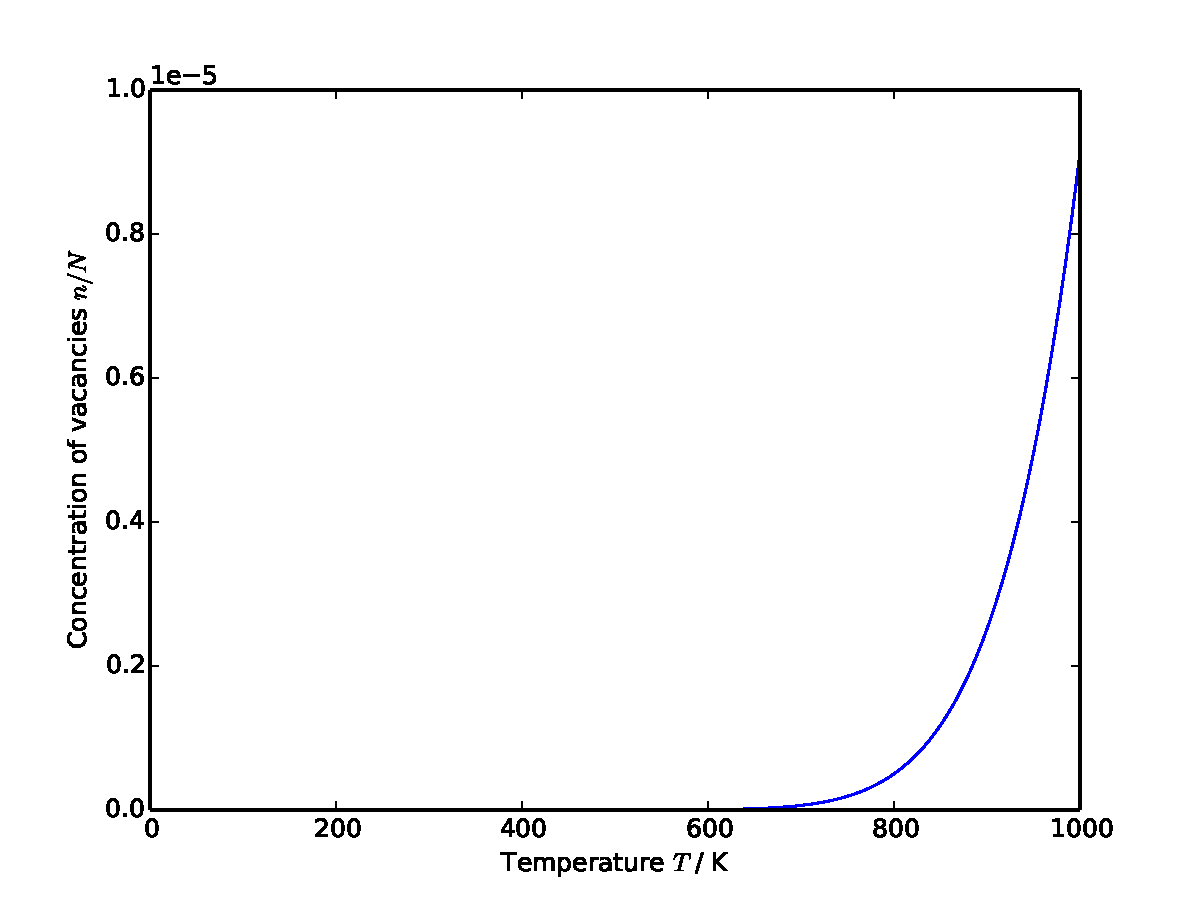
\includegraphics[scale=0.7, clip=true, trim= 0 0 0 0]{FYS2160-oblig-3-fig-conc-n-T.pdf}
				\caption{Concentration of vacancies $n/N$ in the crystal as a function of temperature.}
				\label{fig: concentration of vacancies}
			\end{figure}
		
		
		
		
		\item[h)]
			The heat capacity is defined as
			\begin{align*}
				C_V = \left( \frac{\partial U}{\partial T} \right) _{N,V}
			\end{align*}
			Again, using that the total energy needed to make $n$ vacancies is $U=\epsilon_0+n\Delta \epsilon$. Then $n=(U-\epsilon_0)/\Delta \epsilon$ as above. Eq. \eqref{eq: crystal number of vacancies n(T)} then becomes
			\begin{align*}
				\frac{U-\epsilon_0}{\Delta \epsilon} &= Ne^{-\Delta \epsilon/(kT)} \\
				U &= \Delta \epsilon Ne^{-\Delta \epsilon /(kT)}  + \epsilon_0
			\end{align*}
			so the expression for the specific heat capacity is
			\begin{align*}
				C_V &=  \left( \frac{\partial U}{\partial T} \right) _{N,V} \\
				&= \Delta \epsilon Ne^{-\Delta \epsilon/(kT)} \cdot \frac{\Delta \epsilon}{kT^2} \\
				&= \frac{\Delta \epsilon^2 N}{kT^2}e^{-\Delta \epsilon /(kT)}
			\end{align*}
			Fig. \ref{fig: crystal heat capacity} shows a plot of this in the temperature range from $T=0$ to $T=1000$ K. The heat capacity seems to be very high at high temperatures compared to lower temperatures. Whether or not this is a true behaviour is not easy to say without any experimental data, however, the expression for the heat capacity was derived under the assumption of $n<<N$ - i.e. low temperatures. 1000K may not be a very low temperature.
			\begin{figure}[H]
				\centering
				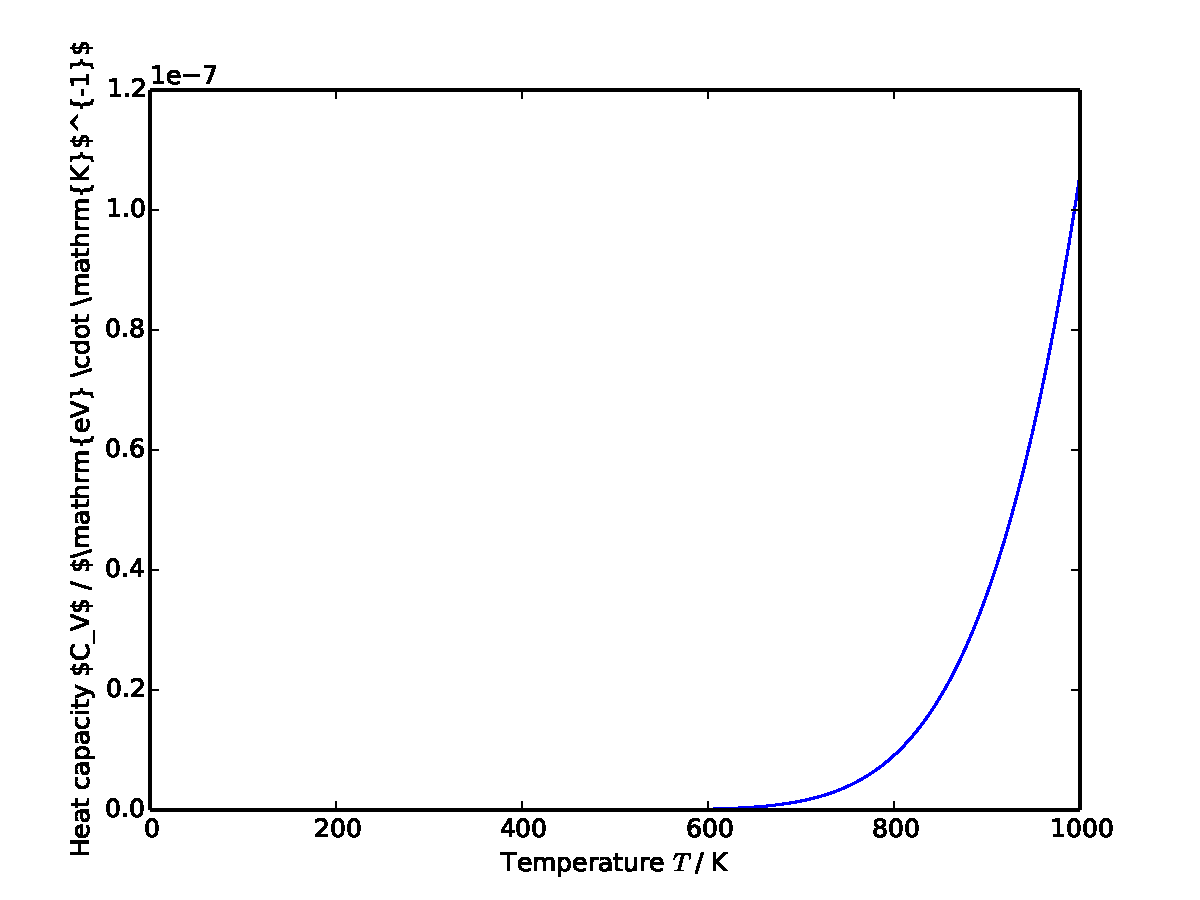
\includegraphics[scale=0.7, clip=true, trim= 0 0 0 0]{FYS2160-oblig-3-fig-heat-capacity.pdf}
				\caption{Specific heat capacity of the crystal as a function of temperature}
				\label{fig: crystal heat capacity}
			\end{figure}
			
			
	\end{itemize}
\end{exercise}



\begin{exercise}
	\begin{itemize}
		\item[a)]
			Since there are $N$ links and $N_R$ of them are pointing to the right, the multiplicity of the mactrostate $N_R$ is
			\begin{align}
				\Omega (N,N_R) = \begin{pmatrix}N \\ N_R\end{pmatrix} = \frac{N!}{N_R!(N-N_R)!} \label{eq: multiplicity polymer exact}
			\end{align}
		
		
		
		\item[b)]
			The total length of the polymer, in terms of $N_R$ and $N_L$ is
			\begin{align*}
				L = \Delta L (N_R - N_L)
			\end{align*}
			when the right-direction is assumed positive. The total number of links is $N$ given by
			\begin{align*}
				N = N_R + N_L \Rightarrow N_L = N - N_R
			\end{align*}
			and so the total length of the polymer is
			\begin{align}
				L = \Delta L (2N_R - N) \label{eq: length of polymer}
			\end{align}
		
		
		
		
		
		\item[c)]
			The entropy is given by
			\begin{align*}
				S = k\ln \Omega(N, N_R)
			\end{align*}
			using eq. \eqref{eq: multiplicity polymer exact} we get
			\begin{align*}
				S	&= k\ln\left( \frac{N}{N_R!(N-N_R)!} \right) \\
					&\approx k\left[ \ln \sqrt{2\pi N} + N\ln N - N - \ln \sqrt{2\pi N_R} - N_R \ln N_R + N_R - \ln \sqrt{2\pi(N-N_R} - (N-N_R)\ln (N-N_R) + (N-N_R) \right]
			\end{align*}
			where I used Stirling's approximation, eq. \eqref{eq: strilings approximation}. With the same argumentation as above, this last equation reduces when $N$, $N_R$ and $N-N_R$ are large. We get
			\begin{align}
				S &\approx k\left[ N\ln N - N_R \ln N_R - (N-N_R)\ln (N-N_R) \right] \label{eq: entropy approx polymer S(N_R)}
			\end{align}
			Rearranging eq. \ref{eq: length of polymer}, we get
			\begin{align}
				N_R = \frac{L+N\Delta L}{2\Delta L} \label{eq: N_R polymer}
			\end{align}
			Using this we obtain the expression for the entropy of the polymer in terms of $N$, $\Delta L$ and $L$:
			\begin{align*}
				S &\approx k \left[ N\ln N - \frac{L+N\Delta L}{2\Delta L}\ln \left( \frac{L+N\Delta L}{2\Delta L} \right) + \frac{N\Delta L - L}{2\Delta L} \ln \left( \frac{N\Delta L - L}{2\Delta L} \right)  \right]
			\end{align*}
		
		
		
		
		\item[d)]
			Since we are dealing with a 2D object, there will not be a change in entropy due to change in volume (and hence pressure), and the number of particles is constant. There will, however, be a change in entropy due to rearranging the links so that more point to the right. Let $\Delta E$ be the change in the systems internal energy. Then the total change in energy is $\Delta U = \Delta E - W$ when $W=F\Delta L$ is the work done when the polymer is stretched. Converting to differentials: $dU = dE - FdL$.
			
			Since the energy is the only thing that can vary, we have
			\begin{align*}
				\Delta S = \left( \frac{\Delta S}{\Delta U} \right) _{N,U} \rightarrow dS = \frac{\partial S}{\partial U} d U = \frac{1}{T}dU
			\end{align*}
			Where I, in the last transition, used the definition of temperature. Inserting the above derived expression for $dU$, we obtain
			\begin{align*}
				TdS = dE - FdL
			\end{align*}
		
		
		
		
		\item[e)]
			Let's assume a process where $dE = 0$. The thermodynamic identity derived in the last exercise then reduces to
			\begin{align*}
				TdS = -FdL \Rightarrow \frac{F}{T} = -\frac{dS}{dL} \rightarrow  -\frac{\partial S}{\partial L}
			\end{align*}
		
			Using this and eq. \eqref{eq: entropy approx polymer S(N_R)} and \eqref{eq: N_R polymer} we obtain an expression for the tension force $F$:
			\begin{align*}
				\frac{F}{T} 	&= -\frac{\partial S}{\partial L} = -\frac{\partial S}{\partial L} \frac{\partial N_R}{\partial N_R} = -\frac{\partial S}{\partial N_R} \frac{\partial N_R}{\partial L} \\
									&= -k\left[ \ln (N-N_R) - \ln N_R \right] \frac{1+N\Delta L}{2\Delta L} \\
									&= -k \ln \left( \frac{N-N_R}{N_R} \right) \left( \frac{1+N\Delta L}{2\Delta L} \right) \\
									&= -k\left( \frac{1+N\Delta L}{2\Delta L} \right) \ln \left( \frac{N\Delta L - L}{N\Delta L + L} \right) \\
									&= -k\left( \frac{1+N\Delta L}{2\Delta L} \right) \left[ \ln \left( N\Delta L \left( 1- \frac{L}{N\Delta L} \right)  \right) -\ln \left( N\Delta L \left( 1+\frac{L}{N\Delta L} \right)  \right)  \right] \\
									&= -k\left( \frac{1+N\Delta L}{2\Delta L} \right) \left[ \ln \left( 1-\frac{L}{N\Delta L} \right) - \ln \left( 1+ \frac{L}{N\Delta L} \right) \right]
			\end{align*}
			Assuming $N\Delta L >> L$, we can use the Taylor expansions
			\begin{align*}
				\ln (1-x) = -x + O(x^2) \qquad \qquad \mathrm{and} \qquad \qquad \ln (1+x) = x + O(x^2)
			\end{align*}
			to simplify:
			\begin{align}
				\frac{F}{T}		&= k\left( \frac{1+N\Delta L}{2\Delta L} \right) \frac{2L}{N\Delta L} \label{eq: F/T polymer}
			\end{align}
			which, for temperatures, obeys Hooke's law: $F \propto L$.
			
			
			
		\item[f)]
			See previous exercise.
		
		\item[g)]
			Eq. \eqref{eq: F/T polymer} tells us that the force in the polymer increases as the temperature increases. In other words, the tension in the polymer increases with temperature. Physically, this is somewhat counter intuitive, for, although at high temperature the polymer obviously looses all elasticity (at which point it looses its characteristics as a polymer as well), one could imagine that the individual strands have a smaller possibility to move at low temperatures, and thereby increasing the tension when force is applied. Why? The answer lies in a combination of the second law of thermodynamics and Gibbs free energy.
		
		\item[h)]
			By stretching the rubber band, one increases the number of links pointing to the right. This, in turn, causes the multiplicity to decrease and thereby the entropy caused by the multiplicity of the direction of the links. To avoid violating the second law of thermodynamics, at least the entropy lost must be gained somewhere else. By raising the temperature, the rubber band accomplishes just that.
	\end{itemize}
\end{exercise}

\begin{bottompar}
\begin{center}
	Oblig \ObligNumber slutt
\end{center}
\end{bottompar}
\end{document}